%% abtex2-modelo-trabalho-academico.tex, v-1.9.5 laurocesar
%% Copyright 2012-2015 by abnTeX2 group at http://www.abntex.net.br/
%%
%% This work may be distributed and/or modified under the
%% conditions of the LaTeX Project Public License, either version 1.3
%% of this license or (at your option) any later version.
%% The latest version of this license is in
%%   http://www.latex-project.org/lppl.txt
%% and version 1.3 or later is part of all distributions of LaTeX
%% version 2005/12/01 or later.
%%
%% This work has the LPPL maintenance status `maintained'.
%%
%% The Current Maintainer of this work is the abnTeX2 team, led
%% by Lauro César Araujo. Further information are available on
%% http://www.abntex.net.br/
%%
%% This work consists of the files abntex2-modelo-trabalho-academico.tex,
%% abntex2-modelo-include-comandos and abntex2-modelo-references.bib
%%

% ------------------------------------------------------------------------
% ------------------------------------------------------------------------
% abnTeX2: Modelo de Trabalho Academico (tese de doutorado, dissertacao de
% mestrado e trabalhos monograficos em geral) em conformidade com
% ABNT NBR 14724:2011: Informacao e documentacao - Trabalhos academicos -
% Apresentacao
% ------------------------------------------------------------------------
% ------------------------------------------------------------------------

\documentclass[
	% -- opções da classe memoir --
	12pt,				% tamanho da fonte
	%openright,			% capítulos começam em pág ímpar (insere página vazia caso preciso)
	openany, % a chapter can start on any page, then many classes support option openany, e.g.:
	%oneside, % With twoside layout (default for class book) chapters start at odd numbered pages and sometimes LaTeX needs to insert a page to ensure this.
	%twoside,			% para impressão em verso e anverso. Oposto a oneside
	a4paper,			% tamanho do papel.
	% -- opções da classe abntex2 --
	%chapter=TITLE,		% títulos de capítulos convertidos em letras maiúsculas
	%section=TITLE,		% títulos de seções convertidos em letras maiúsculas
	%subsection=TITLE,	% títulos de subseções convertidos em letras maiúsculas
	%subsubsection=TITLE,% títulos de subsubseções convertidos em letras maiúsculas
	% -- opções do pacote babel --
	english,			% idioma adicional para hifenização
	french,				% idioma adicional para hifenização
	spanish,			% idioma adicional para hifenização
	brazil				% o último idioma é o principal do documento
	]{abntex2}

% ---
% Pacotes básicos
% ---
\usepackage{lmodern}			% Usa a fonte Latin Modern
\usepackage[T1]{fontenc}		% Selecao de codigos de fonte.
\usepackage[utf8]{inputenc}		% Codificacao do documento (conversão automática dos acentos)
\usepackage{lastpage}			% Usado pela Ficha catalográfica
\usepackage{indentfirst}		% Indenta o primeiro parágrafo de cada seção.
\usepackage{color}				% Controle das cores
\usepackage{graphicx}			% Inclusão de gráficos
\usepackage{microtype} 			% para melhorias de justificação
\usepackage{booktabs}
\usepackage{graphicx}
\usepackage[table,xcdraw]{xcolor}
\usepackage{float}
\usepackage{listings}
\usepackage{ragged2e}


% --- https://www.overleaf.com/learn/latex/Code_listing



\usepackage{xcolor}
\renewcommand\lstlistingname{Lista de código}
\renewcommand\lstlistlistingname{Lista de trechos de código}

% https://tex.stackexchange.com/questions/111580/removing-an-unwanted-page-between-two-chapters
\let\cleardoublepage\clearpage % Unwanted one-page gap between two chapters can be eliminated using the syntax




\definecolor{codegreen}{rgb}{0,0.6,0}
\definecolor{codegray}{rgb}{0.5,0.5,0.5}
\definecolor{codepurple}{rgb}{0.58,0,0.82}
\definecolor{backcolour}{rgb}{0.95,0.95,0.92}

\lstdefinestyle{mystyle}{
    backgroundcolor=\color{backcolour},
    commentstyle=\color{codegreen},
    keywordstyle=\color{magenta},
    numberstyle=\tiny\color{codegray},
    stringstyle=\color{codepurple},
    basicstyle=\ttfamily\footnotesize,
    breakatwhitespace=false,
    breaklines=true,
    captionpos=b,
    keepspaces=true,
    numbers=left,
    numbersep=5pt,
    showspaces=false,
    showstringspaces=false,
    showtabs=false,
    tabsize=2
}

\lstset{style=mystyle}





% ---
% Pacotes adicionais, usados apenas no âmbito do Modelo Canônico do abnteX2
% ---
\usepackage{lipsum}				% para geração de dummy text
% ---

% ---
% Pacotes de citações
% ---
\usepackage[brazilian,hyperpageref]{backref}	 % Paginas com as citações na bibl
\usepackage[alf]{abntex2cite}	% Citações padrão ABNT

% --- checkmark
\usepackage{tikz}
\def\checkmark{\tikz\fill[scale=0.4](0,.35) -- (.25,0) -- (1,.7) -- (.25,.15) -- cycle;} 


% First pip install pygments

% CONFIGURAÇÕES DE PACOTES
% ---

% ---
% Configurações do pacote backref
% Usado sem a opção hyperpageref de backref
\renewcommand{\backrefpagesname}{Citado na(s) página(s):~}
% Texto padrão antes do número das páginas
\renewcommand{\backref}{}
% Define os textos da citação
\renewcommand*{\backrefalt}[4]{
	\ifcase #1 %
		Nenhuma citação no texto.%
	\or
		Citado na página #2.%
	\else
		Citado #1 vezes nas páginas #2.%
	\fi}%
% ---

% ---
% Informações de dados para CAPA e FOLHA DE ROSTO
% ---
\titulo{Relat\'{o}rio Anual PIBi}
\autor{Daniel Terra Gomes}
\local{Campos dos Goytacazes, RJ}
\data{\today, v1.0.0}
%\orientador{Manuel Antonio Molina Palma}
%\coorientador{Equipe \abnTeX}
\instituicao{%
Universidade Estadual do Norte Fluminense Darcy Ribeiro
  \par
  Ciência da Computação
  \par
  INF01205 - IA 2022}
\tipotrabalho{Projeto de Pesquisa}
% O preambulo deve conter o tipo do trabalho, o objetivo,
% o nome da instituição e a área de concentração
\preambulo{Relatório Atividade 1 apresentado ao Curso de Ciência da Computação da
Universidade Estadual do Norte Fluminense
Darcy Ribeiro, como requisito avaliativo da
disciplina.}
% ---

% ---
% Configurações de aparência do PDF final

% alterando o aspecto da cor azul
\definecolor{blue}{RGB}{41,5,195}

% informações do PDF
\makeatletter
\hypersetup{
     	%pagebackref=true,
		pdftitle={\@title},
		pdfauthor={\@author},
    	pdfsubject={\imprimirpreambulo},
	    pdfcreator={LaTeX with abnTeX2},
		pdfkeywords={abnt}{latex}{abntex}{abntex2}{trabalho acadêmico},
		colorlinks=true,       		% false: boxed links; true: colored links
    	linkcolor=blue,          	% color of internal links
    	citecolor=blue,        		% color of links to bibliography
    	filecolor=magenta,      		% color of file links
		urlcolor=blue,
		bookmarksdepth=4
}
\makeatother
% ---

% ---
% Espaçamentos entre linhas e parágrafos
% ---

% O tamanho do parágrafo é dado por:
\setlength{\parindent}{1.3cm}

% Controle do espaçamento entre um parágrafo e outro:
\setlength{\parskip}{0.2cm}  % tente também \onelineskip

% ---
% compila o indice
% ---
\makeindex
% ---

% ----
% Início do documento
% ----
\begin{document}


\begin{center}
\large
\textbf{PROGRAMA INSTITUCIONAL DE BOLSAS DE INICIA\c{C}\~{A}O CIENTIF\'{I}CA E TECNOL\'{O}GICA\\\vspace{0,5cm}
UNIVERSIDADE ESTADUAL DO NORTE FLUMINENSE DARCY RIBEIRO\\
}
\textit{Centro CCT \\
Labotat\'{o}rio LCMAT\\
\vspace{1cm}
Relat\'{o}rio do per\'{\i}odo: Junho 2022 - Maio 2023}\\
\vspace{1,5cm}
\textbf{Relat\'{o}rio Anual PIBi}\\\vspace{5cm}
\end{center}
\textbf{Bolsista}: Daniel Terra Gomes\\
\textbf{Matricula}: 00119110484\\
\textbf{Orientadora}: Prof. Dra. Annabell Del Real Tamariz  \\
\textbf{Curso}: Bacharelado em Ci\^{e}ncia da Computa\c{c}\~{a}o\\
\vspace{3cm}
\begin{center}
\textbf{Titulo do Projeto}: Veículos Autônomos no Brasil e suas tecnologias.\\
\textbf{T\'{\i}tulo do Plano de Trabalho}: Ponta do Iceberg: primeiros passos na Ciência de dados\\
\textbf{Fonte financiadora:} PIBICT/UENF
\end{center}



% Seleciona o idioma do documento (conforme pacotes do babel)
%\selectlanguage{english}
\selectlanguage{brazil}

% Retira espaço extra obsoleto entre as frases.
\frenchspacing

% ----------------------------------------------------------
% ELEMENTOS PRÉ-TEXTUAIS
% ----------------------------------------------------------
% \pretextual

% ---
% Capa
% ---
%%%%%%%%%%%%%%%%%%\%%\\imprimircapa
% ---

% ---
% Folha de rosto
% (o * indica que haverá a ficha bibliográfica)
% ---
%%%%%%%%%%%%%%%%\%%%%\imprimirfolhaderosto*
% ---

% ---
% Inserir a ficha bibliografica
% ---

% Isto é um exemplo de Ficha Catalográfica, ou ``Dados internacionais de
% catalogação-na-publicação''. Você pode utilizar este modelo como referência.
% Porém, provavelmente a biblioteca da sua universidade lhe fornecerá um PDF
% com a ficha catalográfica definitiva após a defesa do trabalho. Quando estiver
% com o documento, salve-o como PDF no diretório do seu projeto e substitua todo
% o conteúdo de implementação deste arquivo pelo comando abaixo:
%
% \begin{fichacatalografica}
%     \includepdf{fig_ficha_catalografica.pdf}
% \end{fichacatalografica}

%\begin{fichacatalografica}
%	\sffamily
%	\vspace*{\fill}					% Posição vertical
%	\begin{center}					% Minipage Centralizado
%	\fbox{\begin{minipage}[c][8cm]{13.5cm}		% Largura
%	\small
%	\imprimirautor
%	%Sobrenome, Nome do autor
%
%	\hspace{0.5cm} \imprimirtitulo  / \imprimirautor. --
%	\imprimirlocal, \imprimirdata-
%
%	\hspace{0.5cm} \pageref{LastPage} p. : il. \\ % (algumas color.) ; 30 cm.\\
%
%	\hspace{0.5cm} \imprimirorientadorRotulo~\imprimirorientador\\
%
%	\hspace{0.5cm}
%	\parbox[t]{\textwidth}{\imprimirtipotrabalho~--~\imprimirinstituicao,
%	\imprimirdata.}\\
%
%	\hspace{0.5cm}
%		1. Veículos autônomos.
%		2. Inteligência Artificial.
%		3. Machine Learning.
%		4. Condução Autônoma.
%		I. Manuel Antonio Molina Palma.
%		II. Universidade Estadual do Norte Fluminense Darcy Ribeiro.
%		III. Faculdade de Ciência da Computação.
%		IV. Veículos autônomos e inteligência artificial:
% um estudo sobre a implementação no brasil.
%	\end{minipage}}
%	\end{center}
%\end{fichacatalografica}
% ---

% ---
% Inserir errata
% ---

% Inserir folha de aprovação
% ---

% Isto é um exemplo de Folha de aprovação, elemento obrigatório da NBR
% 14724/2011 (seção 4.2.1.3). Você pode utilizar este modelo até a aprovação
% do trabalho. Após isso, substitua todo o conteúdo deste arquivo por uma
% imagem da página assinada pela banca com o comando abaixo:
%
% \includepdf{folhadeaprovacao_final.pdf}
%
%%%%%%%%%%\ %%%%%%%%%%\ folhadeaprovacao DELETED

% ---

% ---
% Dedicatória
% ---

% ---
% Agradecimentos
% ---
%%%%\begin{agradecimentos}
%%%%Agradeço aos meus pais que se dedicaram para que eu pudesse estar cursando esta graduação, assim podendo completar mais uma etapa da minha vida.
%%%%Sem o apoio, conselhos, carinho e amor, nada disso seria possível. Sou eternamente grato por tudo que vocês fazem e sempre fizeram para que minha vida fosse especial.
%%%%
%%%%Agradeço ao professor Dr. Manuel Antonio Molina Palma pela dedicação e paciência durante o lecionamento desta disciplina, e obrigado pela ajuda e por estar disponível nos momentos de necessidade.
%%%%
%%%%Por último, mas não menos importante, agradeço a toda minha família e amigos que estiveram comigo em todos os momentos da minha vida.
%%%%
%%%%
%%%%\end{agradecimentos}
% ---

% ---
% Epígrafe
% ---
\begin{epigrafe}
	\vspace*{\fill}
	\begin{flushright}
		\textit{``Behind me lies a farm. \\
			I wonder if there is bread above the hearth \\
			and if I will ever return.'' \\
			(Pantheon, League of Legends)}
	\end{flushright}
\end{epigrafe}
% ---

% ---
% RESUMOS
% ---

% resumo em português
% resumo em inglês



%%%%%%%%%%%
% ---
% inserir lista de ilustrações
% ---
\pdfbookmark[0]{\listfigurename}{lof}
\listoffigures*
\cleardoublepage
% ---

% ---
% inserir lista de tabelas
% ---
%\pdfbookmark[0]{\listtablename}{lot}
%\listoftables*
%\cleardoublepage


% ---

% ---
% inserir lista de abreviaturas e siglas
% ---
\begin{siglas} \label{eq:1}
	\item[VA] Veículo Autônomo 
	\item[VAs] Veículos Autônomos
	\item[ML] Machine Learning
	\item[IA] Inteligência Artificial
	\item[SAE] Society of Automotive Engineers
	\item[ADAS] Advanced Driver-Assistance System
	\item[MaaS] Mobility as a service
	\item[ADS] Automated Driving System
	\item[DDT] Dynamic Driving Task
	\item[ADS-DV] ADS-dedicated vehicle
	\item[2D] Bidimensional
	\item[3D] Tridimensional
	\item[ACC] Adaptive Cruise Control
\end{siglas}

% ---

% ---
% inserir lista de símbolos
% ---


% ---
% inserir o sumario
% ---
\pdfbookmark[0]{\contentsname}{toc}
\tableofcontents*
\cleardoublepage
% ---



% ----------------------------------------------------------
% ELEMENTOS TEXTUAIS
% ----------------------------------------------------------
\textual

% ----------------------------------------------------------
% Introdução (exemplo de capítulo sem numeração, mas presente no Sumário)
% ----------------------------------------------------------
\chapter*[Introdução]{Introdução}
\addcontentsline{toc}{chapter}{Introdução}
% ----------------------------------------------------------

Veículos são partes essenciais de nossas vidas, fazemos uso para ir a universidade, trabalho, escola, compras, viagens, e muito mais. Sendo um dos principais meios de transporte em nossa sociedade.
Desse modo, com o passar do tempo, buscamos maneiras de tornar nossas vidas mais práticas, e automatizadas. A partir destas necessidades surgem os veículos autônomos, que são veículos capazes de fazer sentido do que está ao seu redor e operar sem a necessidade de intervenção humana. Suas principais características são suportar recursos como detecção do ambiente, conexão com a internet, seguir às diretrizes de trânsito, navegar por conta própria em diferentes níveis de automação, tomar decisões de maneira rápidas e eficiente, garantir a segurança de pedestres e passageiros, estacionar, etc.

Veículos autônomos (VAs) e as tecnologias associadas para a execução dos seus recursos ganharam rapidamente a atenção da comunidade de pesquisa e indústria. Portanto, tanto a indústria quanto às comunidades de pesquisa têm trabalhado em abordagens de solução para realizar a direção autônoma de veículos de maneira mais otimizada possível, com foco em enriquecer a percepção do veículo, melhorar a tomada de decisões, implantar e aperfeiçoar a inteligência nos veículos, sofisticar as tecnologias de comunicação para permitir um veículo confiável e com comunicação em tempo real para tudo ao seu redor. Tudo isso fazendo uso de tecnologias sensoriais como: visão computacional, odometria, GPS, lasers, sensores, sistema de mapeamento para navegar, entre outros.

Toda essa atenção, e necessidades de aprimoramento tecnológico faz essa categoria de veículos ganhar, progressivamente, penetração no mercado global. Fazendo com que em 2019 houvesse 31 milhões de máquinas com algum nível de automação em operação em todo o mundo, esse número deve aumentar para 54 milhões até 2024 \cite{sensors}. Mostrando uma tendência em automação de máquinas que antes eram operadas apenas por seres humanos.

Dentre os incentivos para a implementação dessa tecnologia está a diminuição das emissões de CO2 e NO2. Visto que, são veículos unicamente elétricos ou híbridos, não fazem a queima de combustíveis fósseis, levando a diminuição na emissão desses gases. Todavia, há toda uma perspectiva que os VAs, hoje, podem ter uma emissão equivalente a todos os Data Centers em funcionamento, ou 0,3\% das emissões globais. Isso devido ao poder computacional exigido por essas máquinas inteligentes para processar o mundo à sua volta. Todo esse uso de recursos é equivalente a todo o país da Argentina, aproximadamente. Com um computador de controle mais poderoso de 3.100 watts, por exemplo, essas máquinas inteligentes irão emitir mais que o dobro disso, ou cerca de 1\% das emissões globais \cite{intro-pm}.
Além disso, devido ao aumento da consciência ambiental, a sociedade iniciou um processo de endurecimento da legislação nos países ricos contra a emissão de poluentes, o que levou à indústria a promover a geração de energia a partir de fontes renováveis como a energia solar, e no setor de transportes o incentivo a adoção de veículos elétricos.

Ademais, devido à rápida urbanização os congestionamentos se tornaram problemas contínuos para muitos centros urbanos em todo o mundo, levando a atrasos excessivos, poluição sonora e do ar, motoristas frustrados e alto consumo de energia. Os veículos totalmente autônomos vem como uma potencial solução para a solução desse problema. A partir do aumento da capacidade dos VAs de transitar por meio de pelotão de veículos, e, também, com menor impacto na ocupação do solo devido à redução da demanda de vagas de estacionamento disponíveis, além de permitir o acesso básico ao transporte para indivíduos que não podem conduzir veículos, impulsionando e promovendo a equidade entre os cidadãos \cite{conge}.

Os VAs, também, vem como uma solução para a diminuição das mortes no trânsito. Estima-se que no brasil o número de mortes em acidentes de transporte terrestre no período de 2019 foi de 31.945 \cite{Anexo_I_pnatrans}. Além disso, é previsto que até 2030 as colisões fatais no trânsito serão a quinta fonte de mortes nos países em desenvolvimento. 
Os principais fatores de risco em acidentes de trânsito são: excesso de velocidade, direção sob a influência de álcool, distrações, veículos inseguros e infraestrutura insegura das vias \cite{review-auto}.

Em geral, o fator humano é o principal causador de acidentes de trânsito, e os VAs vem como uma solução para isso. Pois, como ja apresentado, são veículos capazes de detectar o ambiente ao redor, planejar o caminho mais curto e seguro, controlar a velocidade, navegar e estacionar sem intervenção de pessoas, reduzindo assim os acidentes por erro humano.
Desse modo, eliminando o fator humano na condução de veículos salvará a vida de muitas pessoas, principalmente nos países em desenvolvimento \cite{mundobrasil}. 

Por fim, apesar das especulações e entusiasmos sobre os VAs, ainda pouco se sabe sobre as implicações no meio ambiente e na sociedade. Assim, os principais objetivos neste relatório de projeto são: apresentar as perspectivas de implementação, esboçar cenários do mercado tecnológico, tecnologias essenciais para operação, e características únicas dos VAs. A fim de enriquecer os conhecimentos sobre esse setor e fornecer algumas direções para o futuro dos VAs no Brasil e no mundo.

O relatório está estruturado da seguinte forma: a seção \ref{Etapas} apresenta as etapas propostas no \textit{plano de trabalho}, enquanto a seção \ref{Objetivos} mostra a principal motivação e objetivos deste estudo. A seção \ref{Metodologia} apresenta a metodologia utilizada neste estudo. A seção \ref{resultados} analisa o impacto dos VAs nos diferentes aspectos investigados neste estudo, discute os principais benefícios e desafios da implantação de VAs em países pelo mundo, e apresenta as tecnologias fundamentais para a operação de VAs. A seção \ref{concl} demonstra os cumprimentos do \textit{plano de trabalho} referente a este relatório. A seção \ref{continuidade} apresenta a perspectiva de continuidade dos estudos do bolsista, de modo a aprimorar seus conhecimentos e aprofundar em partes essenciais para esse estudo. A seção \ref{eventos} apresenta a participação em eventos, cursos e atividades do bolsista. Finalmente, a seção \ref{ass} assinatura do bolsista e da sua orientadora.


Uma lista das principais siglas usadas ao longo do relatório é fornecida na Página \pageref{eq:1}.





% PARTE
% ----------------------------------------------------------
%\part{Preparação da pesquisa}
% ----------------------------------------------------------

% ---
% Capitulo com exemplos de comandos inseridos de arquivo externo
% ---
%\include{abntex2-modelo-include-comandos}


\documentclass{article}
\usepackage[brazil]{babel}

\usepackage[a4paper,top=2cm,bottom=2cm,left=3cm,right=3cm,marginparwidth=1.75cm]{geometry}
% Useful packages
\usepackage{amsmath}
\usepackage{graphicx}
\usepackage[colorlinks=true, allcolors=blue]{hyperref}
\usepackage{minted}
\usepackage{float}
\usepackage{soul}
\usepackage{booktabs}
\usepackage{graphicx}
\usepackage[table,xcdraw]{xcolor}

\usepackage{lmodern}	% Usa a fonte Latin Modern
\usepackage[utf8]{inputenc}		% Codificacao do documento (conversão automática dos acentos)




% Pacotes de citações
% ---
\usepackage[brazilian,hyperpageref]{backref}	 % Paginas com as citações na bibl
\usepackage[alf]{abntex2cite}	% Citações padrão ABNT


% First pip install pygments

% CONFIGURAÇÕES DE PACOTES
% ---

% Configurações do pacote backref
% Usado sem a opção hyperpageref de backref
\renewcommand{\backrefpagesname}{Citado na(s) página(s):~}
% Texto padrão antes do número das páginas
\renewcommand{\backref}{}
% Define os textos da citação
\renewcommand*{\backrefalt}[4]{
	\ifcase #1 %
		Nenhuma citação no texto.%
	\or
		Citado na página #2.%
	\else
		Citado #1 vezes nas páginas #2.%
	\fi}%
% --


\title{Plano de trabalho 2022}
\author{Daniel Terra Gomes}

\begin{document}
\begin{titlepage}
\begin{center}
\large
\textbf{PROGRAMA INSTITUCIONAL DE BOLSAS DE INICIA\c{C}\~{A}O CIENTIF\'{I}CA E TECNOL\'{O}GICA\\\vspace{0,5cm}
UNIVERSIDADE ESTADUAL DO NORTE FLUMINENSE DARCY RIBEIRO\\
}
\textit{Centro CCT \\
Labotat\'{o}rio LCMAT\\
\vspace{1cm}}
%Plano de trabalho para o segundo ano da bolsa }\\
\vspace{1,5cm}
\textbf{Plano de Trabalho para Renovação de Bolsa de Iniciação Científica}\\\vspace{5cm}
\end{center}
\textbf{Bolsista}: Daniel Terra Gomes\\
\textbf{Matricula}: 00119110484\\
\textbf{Orientadora}: Prof. Dra. Annabell Del Real Tamariz  \\
\textbf{Curso}: Bacharelado em Ci\^{e}ncia da Computa\c{c}\~{a}o\\
\vspace{3cm}
\begin{center}
\textbf{Titulo do Projeto}: Project-driven Data Science: Aprendendo e Mapeando\\
\textbf{T\'{\i}tulo do Plano de Trabalho}: Dirigindo para o futuro: Softwares e Algoritmos avançados que alimentam Veículos Autônomos.
%Os principais obstáculos para Veículos Autônomos no Brasil, e suas tecnologias essenciais.\\

\textbf{Fonte financiadora:} PIBICT/UENF
\end{center}
\end{titlepage}


%\maketitle
\section{Justificativa}

Os veículos autônomos (VAs) estão revolucionando o transporte e a mobilidade autônoma nos últimos anos, prometendo aumentar a segurança nas estradas, melhorar a eficiência do tráfego, reduzir as emissões de gases de efeito estufa, aumentar acessibilidade dos cidadãos ao transporte público e privado, agilizar o transporte de encomendas e muito mais \cite{review-auto, intro-pm, mundobrasil}.


Logo, para que esses veículos atinjam todo o seu potencial revolucionário, é necessário pesquisas significativas relacionadas a questões organizacionais e tecnológicas para que os VAs atinjam melhores níveis de difusão social \cite{noauthor_undated-mw}, e o seu mais alto nível de automação, ou seja, nível 5 SAE \cite{SAE}. Visto que, como já estudado no primeiro ano de Iniciação Científica \cite{my-work-on-git}, para alcançar maior apoio organizacional e social, e melhores níveis de automação, um veículo autônomo (VA) necessita de: melhores sensores, conexão móvel, computação de borda móvel, melhores algoritmos de aprendizado de máquina, análise de dados, aprendizado distribuído, além da aceitação do público e um melhor amparo legislativo para que essa tecnologia seja extensamente utilizada pela sociedade \cite{KPMG}, e que, também, seja capaz de, por exemplo, compreender o ambiente a sua volta e identificar o estado atual dos agentes próximos de maneira acurada \cite{sensors-yet}.


No entanto, quando se trata de operação segura, acurada e eficiente nas vias, é necessário ir além, um VA não deve apenas entender o estado atual dos agentes próximos, mas também antecipar proativamente o comportamento, comunicar e interpretar intenções e estados dos usuários e objetos na redondeza \cite{conge}. Considerando que, uma parte considerável dessa interpretação, geralmente é prever o comportamento dos pedestres, veículos e sinalizações (ou, de modo geral, dos usuários vulneráveis das vias) \cite{software-review}.


Essa capacidade de identificação, compreensão e interpretação do ambiente são partes fundamentais dos componentes de um VA, sendo esses: percepção, planejamento e controle \cite[p. ~37]{my-work-on-git}. Que são componentes operados e gerenciados por softwares e algoritmos que trabalham no controle do veículo, a partir do computador central, cujo fica encarregado de processar os dados oriundos dos diversos sensores espalhados pelo VA \cite[p. ~39]{my-work-on-git}.


Sabendo disso, temos como objetivo (seção \ref{objetivo}) buscar uma familiarização e compreensão do estado atual das pesquisas e projetos em detecção de ambiente, detecção de pedestres, planejamento de caminhos, e controle de movimento veicular para veículos autônomos a partir da testagem dos principais algoritmos encontrados (elaborado na seção \ref{Metodologia} e \ref{etapas}). Visto que, como pesquisado e estudado no primeiro ano de projeto \cite{my-work-on-git}, fazem parte das \textit{Tecnologias Essenciais para a Direção Autônoma} e mais especificamente das \textit{Arquiteturas, Algoritmos e Softwares} de VAs, cujo será a delimitação desse segundo ano de projeto.


\section{Objetivos} \label{objetivo}
Temos como objetivo desta pesquisa a familiarização e compreensão dos principais softwares e algoritmos de controle de Veículos Autônomos.



\section{Metodologia} \label{Metodologia}
Utilizaremos uma metodologia, com o propósito de revisar a literatura existente, cuja essência é desenvolver e colocar as pessoas envolvidas em contato direto com todo material já desenvolvido em relação a esta iniciação científica, que será constituída principalmente de: artigos científicos, cursos online, publicações em periódicos, jornais online, monografias, dissertações e vídeo aulas.

Nesse formato metodológico, pesquisa bibliográfica, será possível ter contato e se fundamentar com os principais materiais da atualidade relacionados a Veículos Autônomos e seus Algoritmos de Controle, de modo a ter contato com o que há de mais recente sobre o assunto.


Atrelado ao que foi apresentado, seguiremos um princípio metodológico chamado \textit{“Project-based learning”}\footnote{Aprendizagem baseada em projetos} \cite{krajcik2006project}, que visa construir soluções a partir de problemas reais em nossa sociedade. Visto que, é uma modalidade de estudo que deixa as pessoas envolvidas livres para seguir a sua curiosidade, desejo de resolver os problemas encontrados pelo caminho e de buscar por mais informações para resolvê-los. Contemplando assim os objetivos desejados para a realizar de maneira satisfatória deste projeto. 

Além disso, as pesquisas realizadas serão fundamentadas no método de pesquisa \textit{Revisão Sistemática de Literatura} (RSL) que segundo Maria Cristiane (Universidade de São Paulo) \cite{revi3}, e Davi Nakano (Universidade de São Paulo) \cite{revi2} refere-se a um tipo de investigação que se concentra em uma questão bem definida, visando identificar, selecionar, avaliar e sintetizar as evidências disponíveis relacionadas a uma questão formulada de interesse para o pesquisador.

Desse modo, amparado de todo esse ferramental teórico apresentado, seguiremos o seguinte passa a passo:



\begin{enumerate}
\item Primeiro faremos uma pesquisa e levantamento Bibliográfico de modo a agrupar e selecionar os materiais relevantes para este projeto, que será desenvolvida através dos seguintes meios na internet (Google academic, Google livros, biblioteca virtual, jornais virtuais, site das bibliotecas de universidades, plataforma CAPES, YouTube e outros). A busca nesses bancos de dados contemplará os anos de 2022 a 2023. Contudo, também, podemos recorrer a materiais publicados há mais tempo por falta de referenciais melhores. Como palavra-chave empregaremos os termos: Autonomous Vehicles Software, Autonomous, Cars, Mobility, Connected Car, AV, TaxiBot, Self-driving cars, Algorithmus, Deep Learning, Computer Vision, entre outros.  A pesquisa irá se limitar aos idiomas: alemão, inglês, português, e podendo se estender até ao espanhol e francês.

\item De maneira seguinte, faremos a testagem dos algoritmos mais importantes encontrados, de modo a compreendermos os seus funcionamentos. Esses testes se limitaram aos algoritmos relacionados ao controle e autonomia dos veículos autônomos. Recorreremos a repositórios de códigos online para o armazenamento desses algoritmos, e os testes serão realizados em uma máquina local. Ressaltamos que, não nos limitaremos a linguagens de programação, e daremos prioridade a algoritmos e softwares de livre acesso.
\item Por fim, elaboraremos o relatório final usando os matérias encontrados, e dos resumos e rascunhos feitos ao longo das pesquisas.
\end{enumerate}

A elaboração desse projeto terá as seguintes etapas ilustradas na Figura \ref{img_bibli}:

\begin{figure}[H]
\centering
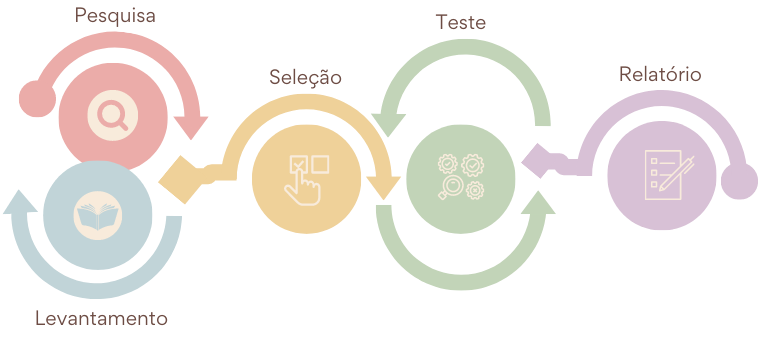
\includegraphics[width=14cm]{Figures/methodology.png}
\caption{Etapas do projeto. Autoral.}
\label{img_bibli}
\end{figure}

\section{Etapas} \label{etapas}
A fim de alcançar os objetivos (seção \ref{objetivo}) do Projeto de Pesquisa, nesta seção do \textit{Plano de Trabalho} listamos as principais atividades que serão realizadas:


\begin{enumerate}
    \item Pesquisa bibliográfica sobre softwares de controle para veículos autônomos;
    \item Levantamento bibliográfico algoritmos de controle de Veículos Autônomos;
    \item Seleção dos principais algoritmos achados no levantamento bibliográfico;
    \item Teste de alguns dos principais dos algoritmos achados;
    \item Elaboração do Relatório Final.
\end{enumerate}

\section{Cronograma das atividades}
Este cronograma visa mostrar o desenvolvimento das atividades listadas na seção \ref{etapas} e ilustrada na Figura \ref{img_bibli}, cada etapa (seção \ref{etapas}) foi dividida de modo a otimizar o tempo e as necessidades do projeto.
% Please add the following required packages to your document preamble:
% \usepackage{booktabs}
% \usepackage{graphicx}
% \usepackage[table,xcdraw]{xcolor}
% If you use beamer only pass "xcolor=table" option, i.e. \documentclass[xcolor=table]{beamer}
\begin{table}[H]
\centering
\resizebox{\textwidth}{!}{%
\begin{tabular}{@{}l|l|l|l|l|l|l|l|l|l|l|l|l|@{}}

\cmidrule(l){1-13}


  \multicolumn{1}{|c|}{\textbf{Etapas/Mês}} &
  \multicolumn{1}{c|}{\textbf{1º}} &
  \multicolumn{1}{c|}{\textbf{2º}} &
  \multicolumn{1}{c|}{\textbf{3º}} &
  \multicolumn{1}{c|}{\textbf{4º}} &
  \multicolumn{1}{c|}{\textbf{5º}} &
  \multicolumn{1}{c|}{\textbf{6º}} &
  \multicolumn{1}{c|}{\textbf{7º}} &
  \multicolumn{1}{c|}{\textbf{8º}} &
  \multicolumn{1}{c|}{\textbf{9º}} &
  \multicolumn{1}{c|}{\textbf{10º}} &
  \multicolumn{1}{c|}{\textbf{11º}} &
  \multicolumn{1}{c|}{\textbf{12º}} \\ \midrule

 
\multicolumn{1}{|l|}{\textbf{1}} 

\cellcolor[HTML]{A4C2F4}&
   &
  \cellcolor[HTML]{A4C2F4} &
  \cellcolor[HTML]{A4C2F4} &
   &
   &
   &
   &
   &
   &
   &
   &
   \\ \midrule
\multicolumn{1}{|l|}{\textbf{2}} &
   &
   &
  \cellcolor[HTML]{A4C2F4} &
  \cellcolor[HTML]{A4C2F4} &
  \cellcolor[HTML]{A4C2F4} &
   &
   &
   &
   &
   &
   &
   \\ \midrule
\multicolumn{1}{|l|}{\textbf{3}} &
   &
   &
   &
   &
   &
   \cellcolor[HTML]{A4C2F4}&
   \cellcolor[HTML]{A4C2F4}&
   &
   &
   &
   &
   \\ \midrule
\multicolumn{1}{|l|}{\textbf{4}} &
   &
   &
   &
&
   &
   &
   &
  \cellcolor[HTML]{A4C2F4} &
   \cellcolor[HTML]{A4C2F4}&
  \cellcolor[HTML]{A4C2F4} &
   &
   \\ \midrule
\multicolumn{1}{|l|}{\textbf{5}} &
   &
   &
  &
   &
   &
   &
   &
   \cellcolor[HTML]{A4C2F4}
   &
   \cellcolor[HTML]{A4C2F4}
   &
  \cellcolor[HTML]{A4C2F4} 
  &
  \cellcolor[HTML]{A4C2F4} 
  &
  \cellcolor[HTML]{A4C2F4} \\ 
  \bottomrule
  
\end{tabular}%
}
\caption{Etapas do Cronograma de atividades}
\label{tab:etapas}
\end{table}

%\centering
%\bibliographystyle{alpha}
\bibliography{bibli}
\end{document}


% ---

% ----------------------------------------------------------
% PARTE
% ----------------------------------------------------------
%\part{Referenciais teóricos}
% ----------------------------------------------------------

% ---
% Capitulo de revisão de literatura

% ---



% ----------------------------------------------------------
% PARTE
% ----------------------------------------------------------
%\part{Resultados}
% ----------------------------------------------------------

% ---
% primeiro capitulo de Resultados
% ---

% ---

% ---


% ---
% segundo capitulo de Resultados
% ---


% ----------------------------------------------------------
% Finaliza a parte no bookmark do PDF
% para que se inicie o bookmark na raiz
% e adiciona espaço de parte no Sumário
% ----------------------------------------------------------
\phantompart

% ---
% Conclusão
% ---
%\chapter{Conclusão}
% ---


% ----------------------------------------------------------
% ELEMENTOS PÓS-TEXTUAIS
% ----------------------------------------------------------
\postextual
% ----------------------------------------------------------

% ----------------------------------------------------------
% Referências bibliográficas
% ----------------------------------------------------------
\bibliography{bibli}



% ----------------------------------------------------------
% Glossário
% ----------------------------------------------------------
%
% Consulte o manual da classe abntex2 para orientações sobre o glossário.
%
%\glossary

% ----------------------------------------------------------
% Apêndices
% ----------------------------------------------------------

% ---
% Inicia os apêndices
%---------------------------------------------------------------------
% INDICE REMISSIVO
%---------------------------------------------------------------------
\phantompart
\printindex
%---------------------------------------------------------------------

\end{document}
